% !TEX TS-program = pdflatex
% !TEX encoding = UTF-8 Unicode

% Example of the Memoir class, an alternative to the default LaTeX classes such as article and book, with many added features built into the class itself.

%\documentclass[12pt,a4paper]{memoir} % for a long document
\documentclass[12pt,a4paper,article]{memoir} % for a short document

\usepackage[utf8]{inputenc} % set input encoding to utf8
\usepackage{graphicx}
\usepackage{pdfpages}

% Don't forget to read the Memoir manual: memman.pdf

%%% Examples of Memoir customization
%%% enable, disable or adjust these as desired

%%% PAGE DIMENSIONS
% Set up the paper to be as close as possible to both A4 & letter:
\settrimmedsize{11in}{210mm}{*} % letter = 11in tall; a4 = 210mm wide
\setlength{\trimtop}{0pt}
\setlength{\trimedge}{\stockwidth}
\addtolength{\trimedge}{-\paperwidth}
\settypeblocksize{*}{\lxvchars}{1.618} % we want to the text block to have golden proportionals
\setulmargins{50pt}{*}{*} % 50pt upper margins
\setlrmargins{*}{*}{1.618} % golden ratio again for left/right margins
\setheaderspaces{*}{*}{1.618}
\checkandfixthelayout 
% This is from memman.pdf

%%% \maketitle CUSTOMISATION
% For more than trivial changes, you may as well do it yourself in a titlepage environment
\pretitle{\begin{center}\sffamily\huge\MakeUppercase}
\posttitle{\par\end{center}\vskip 0.5em}

%%% ToC (table of contents) APPEARANCE
\maxtocdepth{subsection} % include subsections
\renewcommand{\cftchapterpagefont}{}
\renewcommand{\cftchapterfont}{}     % no bold!

%%% HEADERS & FOOTERS
\pagestyle{ruled} % try also: empty , plain , headings , ruled , Ruled , companion

%%% CHAPTERS
\chapterstyle{hangnum} % try also: default , section , hangnum , companion , article, demo

\renewcommand{\chaptitlefont}{\Huge\sffamily\raggedright} % set sans serif chapter title font
\renewcommand{\chapnumfont}{\Huge\sffamily\raggedright} % set sans serif chapter number font

%%% SECTIONS
\hangsecnum % hang the section numbers into the margin to match \chapterstyle{hangnum}
\maxsecnumdepth{subsection} % number subsections

\setsecheadstyle{\Large\sffamily\raggedright} % set sans serif section font
\setsubsecheadstyle{\large\sffamily\raggedright} % set sans serif subsection font

%% END Memoir customization

\title{Manuel d'Utilisation du Web Service Pays d'Étamine}
\author{Team Etamine}
\date{} % Delete this line to display the current date

%%% BEGIN DOCUMENT
\begin{document}

\maketitle
\break
\tableofcontents % the asterisk means that the contents itself isn't put into the ToC

\chapter{Webservice}

\section{Demarrage}
Pour démarrer le web service pays pour Étamine, il est nécessaire de lancer la classe Application.java.\\

\section{Modification du port d'écoute}
Pour modifier le port d'écoute du web service, il suffit de modifier la valeur "" dans le fichier application.properties.\\

\chapter{Client JAVA}

Ce client est prévu pour des developpeurs Java.\\
Il est destiné à être integré à une autre application.\\
Il n'y donc pas d'utilisation directe possible excepté par le biais des classes de test.\\

\chapter{Client PHP}

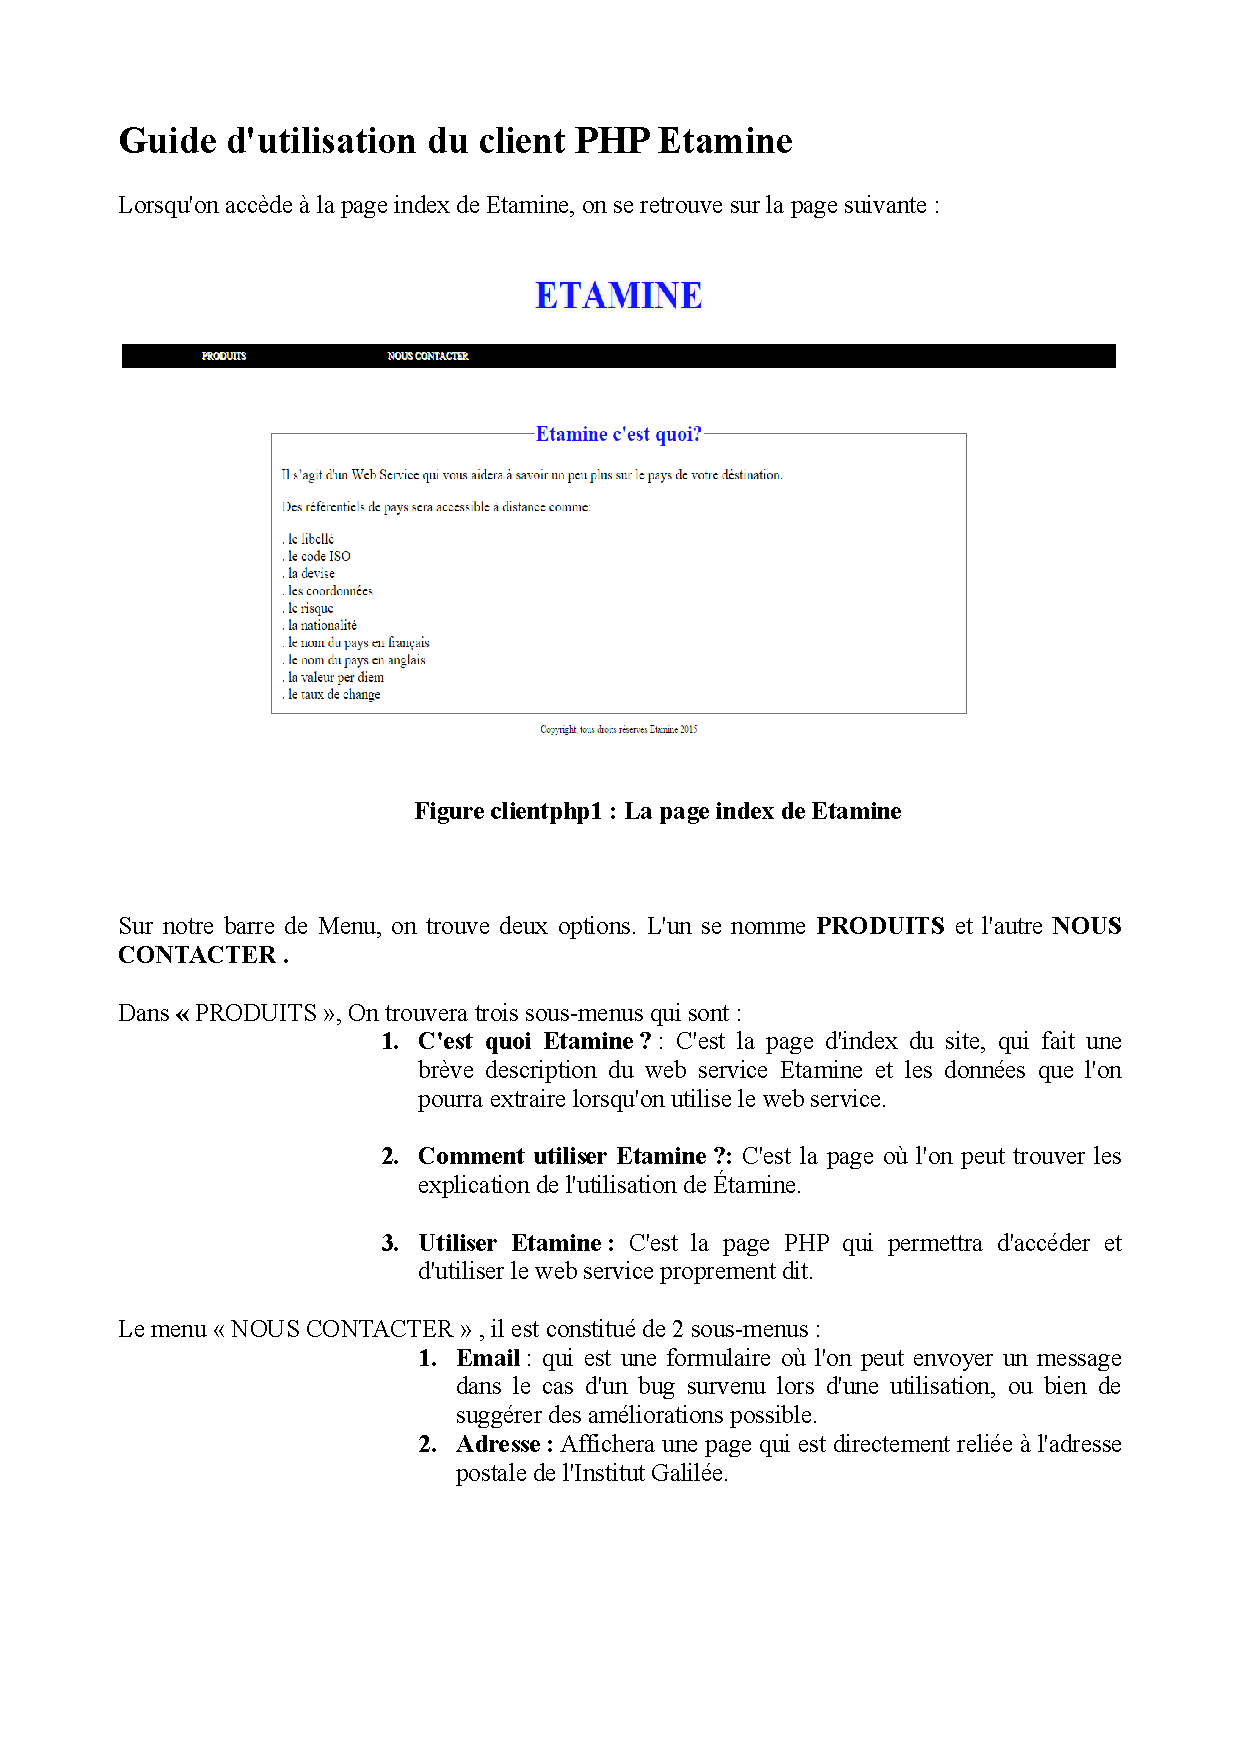
\includepdf[pages = 1-8]{images/ClientPHP}

\chapter{Application de Gestion}

\section{Demarrage}
Pour démarrer l'application de gestion, il faut lancer la classe Application.java.\\

\section{Connexion}
Afin de se connecter à l'application de gestion, il est nécessaire de rentrer un nom d'utilisateur et un mot de passe valide avant de cliquer sur le bouton login.\\ 

\section{Ajouter un pays}
Pour ajouter un pays, il faut cliquer sur le bouton Ajouter un pays.\\
Il faut ensuite remplir les champs concernant le pays à ajouter.\\
Il faut enfin cliquer sur le bouton ajouter pour ajouter le pays.\\

\section{Supprimer un pays}
Pour supprimer un pays, il faut cliquer sur le bouton Supprimer un pays.\\
Il faut ensuite choisir le pays à supprimer.\\
Il faut enfin cliquer sur le bouton supprimer pour ajouter le pays.\\

\section{Modifier un pays}
Pour modifier un pays, il faut cliquer sur le bouton Modifier un pays.\\
Il faut ensuite changerr les champs concernant le pays à modifier.\\
Il faut enfin cliquer sur le bouton modifier pour modifier le pays.\\
\end{document}
